\section{Central Limit Theorem (Teorema del Limite Centrale)}

Per spiegare questo concetto utilizziamo una versione semplificata della \textbf{Galton Board}:

\begin{center}
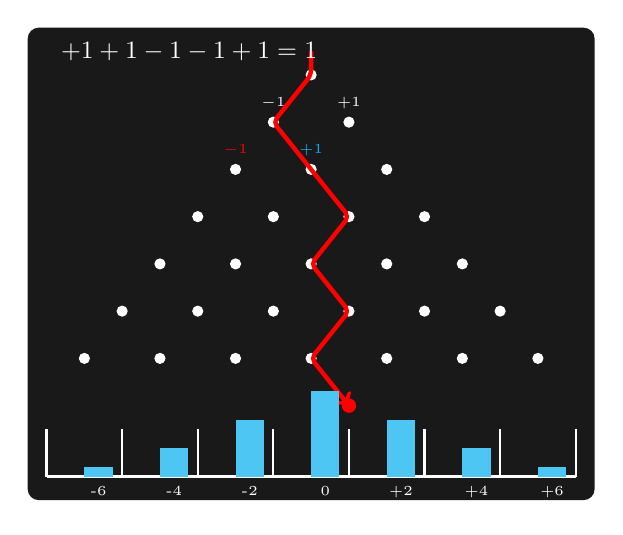
\begin{tikzpicture}[scale=0.6]
    % Sfondo scuro per simulare lo screen
    \fill[black!90, rounded corners] (-6, 1) rectangle (6, -9);
    
    % Pioli (Pegs)
    \foreach \y in {0,...,6} {
        \foreach \x in {0,...,\y} {
            \filldraw[white] (-\y*0.8 + \x*1.6, -\y) circle (3pt);
        }
    }
    
    % Indicazioni +1 / -1
    \node[white, font=\tiny] at (-0.8, -0.6) {$-1$};
    \node[white, font=\tiny] at (0.8, -0.6) {$+1$};
    \node[red, font=\tiny] at (-1.6, -1.6) {$-1$};
    \node[cyan, font=\tiny] at (0, -1.6) {$+1$};
    
    % Traiettoria pallina rossa (esempio)
    \draw[red, ultra thick, ->, rounded corners=2pt] (0, 0.5) -- (0,0) -- (-0.8,-1) -- (0,-2) -- (0.8,-3) -- (0,-4) -- (0.8,-5) -- (0,-6) -- (0.8,-7);
    \filldraw[red] (0.8, -7) circle (4pt);
    
    % Testo in alto
    \node[white, anchor=west, font=\small] at (-5.5, 0.5) {$+1+1-1-1+1=1$};
    
    % Secchielli (Buckets) in basso
    \foreach \i in {-3,...,3} {
        \draw[white, thick] (\i*1.6 - 0.8, -7.5) -- (\i*1.6 - 0.8, -8.5);
    }
    \draw[white, thick] (4*1.6 - 0.8, -7.5) -- (4*1.6 - 0.8, -8.5);
    \draw[white, thick] (-3*1.6 - 0.8, -8.5) -- (4*1.6 - 0.8, -8.5);
    
    % Istogramma approssimato nei secchielli
    \fill[cyan!70] (-3*1.6, -8.5) rectangle ++(0.6, 0.2);
    \fill[cyan!70] (-2*1.6, -8.5) rectangle ++(0.6, 0.6);
    \fill[cyan!70] (-1*1.6, -8.5) rectangle ++(0.6, 1.2);
    \fill[cyan!70] (0, -8.5) rectangle ++(0.6, 1.8);
    \fill[cyan!70] (1*1.6, -8.5) rectangle ++(0.6, 1.2);
    \fill[cyan!70] (2*1.6, -8.5) rectangle ++(0.6, 0.6);
    \fill[cyan!70] (3*1.6, -8.5) rectangle ++(0.6, 0.2);
    
    % Label asse x
    \foreach \i/\val in {-3/-6, -2/-4, -1/-2, 0/0, 1/+2, 2/+4, 3/+6} {
        \node[white, font=\tiny, below] at (\i*1.6+0.3, -8.5) {\val};
    }
\end{tikzpicture}
\end{center}

Una pallina cade su un piolo (la prima volta sul centrale) e ha il 50\% di possibilità di andare a sx o a dx. Ipotizziamo che se la pallina va a sx sottraiamo 1, se va a dx lo aggiungiamo. Ripetiamo questo processo ipotizzando di avere 5 righe di pioli. 

Una pallina fa 5 salti, la sua posizione finale è la somma dei numeri. 
Se ipotizziamo di lanciare tante palline, siamo in grado di capire quanto è probabile un bucket rispetto agli altri. In questo semplice caso possiamo calcolare la probabilità di cadere in un bucket.

Ipotizziamo di avere dei dadi, di lanciarli e di sommarne i valori, non ci interessa della distribuzione, possono essere sia truccati che onesti. Ipotizziamo di sommare 2 dadi, 5, 10, 15:
Possiamo osservare che quanti più dadi lanciamo contemporaneamente, (per lo stesso numero di iterazioni) più è visibile la curva a campana $\sim$.

\begin{center}
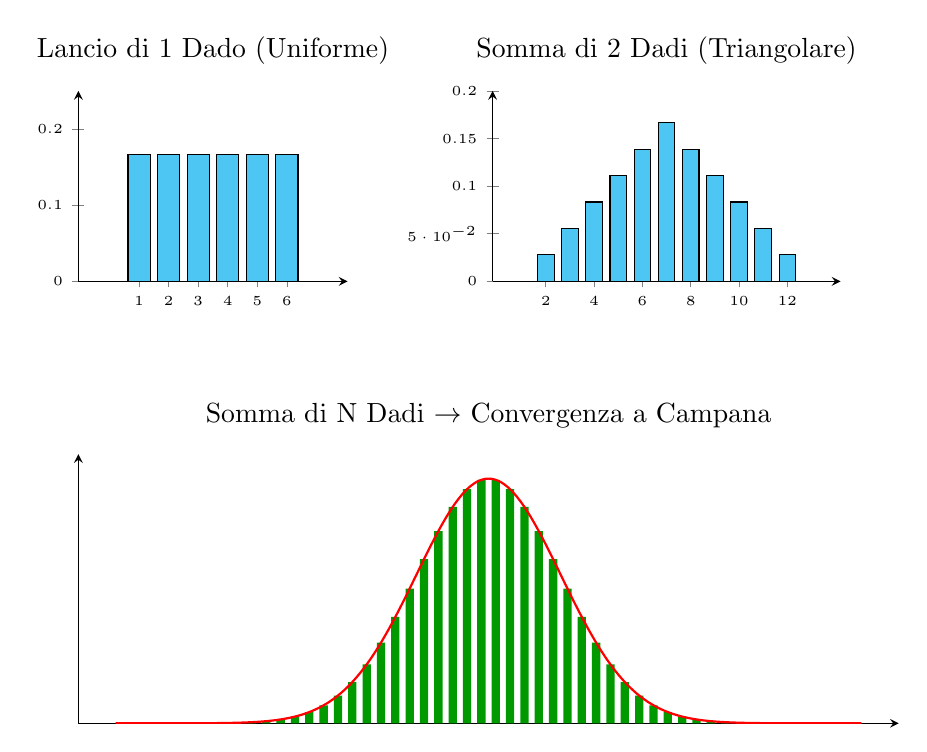
\begin{tikzpicture}
    % Istogramma 1: 1 Dado (Uniforme)
    \begin{axis}[
        name=plot1,
        width=5cm, height=4cm,
        ybar, bar width=8pt,
        title={Lancio di 1 Dado (Uniforme)},
        ymin=0, ymax=0.25, xmin=0, xmax=7,
        xtick={1,2,3,4,5,6},
        axis x line=bottom, axis y line=left,
        enlarge x limits=0.15,
        tick label style={font=\tiny}
    ]
        \addplot[fill=cyan!70] coordinates {(1,1/6) (2,1/6) (3,1/6) (4,1/6) (5,1/6) (6,1/6)};
    \end{axis}
    
    % Istogramma 2: 2 Dadi (Triangolare)
    \begin{axis}[
        name=plot2,
        at={(plot1.right of south east)}, anchor=left of south west,
        width=6cm, height=4cm,
        ybar, bar width=6pt,
        title={Somma di 2 Dadi (Triangolare)},
        ymin=0, ymax=0.2, xmin=1, xmax=13,
        xtick={2,4,6,8,10,12},
        axis x line=bottom, axis y line=left,
        enlarge x limits=0.1,
        tick label style={font=\tiny}
    ]
        \addplot[fill=cyan!70] coordinates {(2,1/36) (3,2/36) (4,3/36) (5,4/36) (6,5/36) (7,6/36) (8,5/36) (9,4/36) (10,3/36) (11,2/36) (12,1/36)};
    \end{axis}
    
    % Istogramma 3: Tanti dadi (Campana)
    \begin{axis}[
        at={(plot1.below south west)}, anchor=above north west, yshift=-1cm,
        width=12cm, height=5cm,
        ybar, bar width=3pt,
        title={Somma di N Dadi $\to$ Convergenza a Campana},
        ymin=0, ymax=1.1, xmin=0, xmax=40,
        xtick=\empty, ytick=\empty,
        axis x line=bottom, axis y line=left,
        enlarge x limits=0.05
    ]
        % Dati approssimati per simulare una gaussiana con N alto (SINTASSI CORRETTA)
        \addplot[fill=green!60!black, draw=none, samples=40, domain=5:35] {exp(-(x-20)^2 / 30)};
        % Disegno la curva limite sopra (SINTASSI CORRETTA)
        \addplot[thick, red, smooth, samples=100, domain=0:40] {exp(-(x-20)^2 / 30)};
    \end{axis}
\end{tikzpicture}
\end{center}

Da una distribuzione asimmetrica oppure una distribuzione simmetrica. \textbf{Questo è vero per qualsiasi distribuzione.}

Vogliamo capire dopo quanto queste distribuzioni convergono ad una Gaussiana. Il modo più semplice per osservarlo è partire da una distribuzione uniforme (es: lancio di un dado).
Ipotizziamo di voler sapere la probabilità di ottenere un numero (somma) lanciando due dadi: contiamo quante coppie fanno quel numero.

\begin{center}
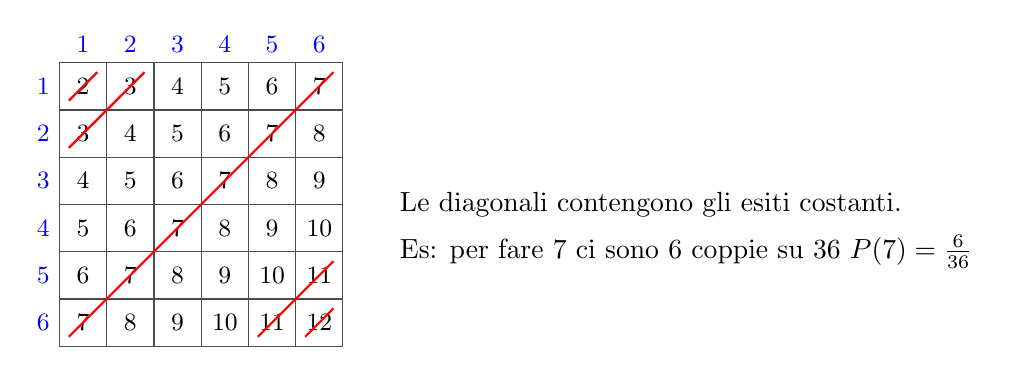
\begin{tikzpicture}[scale=0.6]
    % Matrice delle somme dei due dadi
    \draw[step=1cm, white!30!black, thin] (0,0) grid (6,6);
    
    % Assi esterni
    \foreach \x in {1,...,6} \node[above, font=\small, text=blue] at (\x-0.5, 6) {\x};
    \foreach \y in {1,...,6} \node[left, font=\small, text=blue] at (0, 6-\y+0.5) {\y};
    
    % Riempimento valori (UTILIZZO DI \mysum INVECE DI \sum PER EVITARE CONFLITTI)
    \foreach \x in {1,...,6} {
        \foreach \y in {1,...,6} {
            \pgfmathsetmacro{\mysum}{int(\x+\y)}
            \node[font=\small] at (\x-0.5, 6-\y+0.5) {\mysum};
        }
    }
    
    % Evidenziamo le diagonali (isolinee della somma)
    \draw[red, thick] (0.2, 5.2) -- (0.8, 5.8); % Somma = 2
    \draw[red, thick] (0.2, 4.2) -- (1.8, 5.8); % Somma = 3
    \draw[red, thick] (0.2, 0.2) -- (5.8, 5.8); % Diagonale principale (somma=7)
    \draw[red, thick] (4.2, 0.2) -- (5.8, 1.8); % Somma = 11
    \draw[red, thick] (5.2, 0.2) -- (5.8, 0.8); % Somma = 12
    
    \node[anchor=west] at (7, 3) {Le diagonali contengono gli esiti costanti.};
    \node[anchor=west] at (7, 2) {Es: per fare 7 ci sono 6 coppie su 36 $\implies P(7) = \frac{6}{36}$};
\end{tikzpicture}
\end{center}

È facile da osservare per 3 dadi. Diventa difficile se la distribuzione cambia. 
\textbf{Questa cosa si chiama convoluzione.}

\subsection{Momenti della somma}

Il valore atteso del lancio di un dado è $\mu$. Il valore atteso del lancio di due dadi sommati è $2\mu$, per 3 dadi è $3\mu$ ecc.

\begin{center}
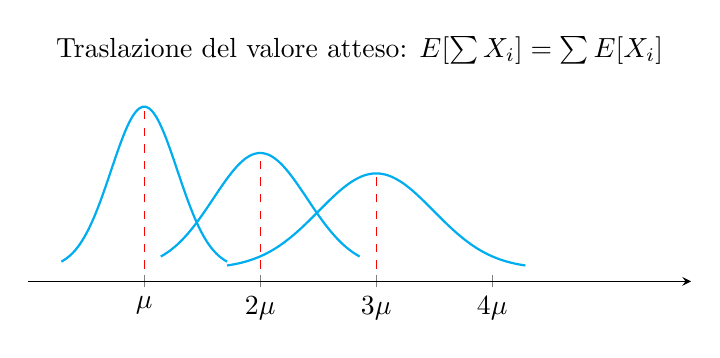
\begin{tikzpicture}
    % Mostriamo come si sposta la media
    \begin{axis}[
        width=10cm, height=4cm,
        axis x line=bottom,
        axis y line=none, % Nascondiamo l'asse y per evitare il warning
        xmin=0, xmax=20,
        xtick={3.5, 7, 10.5, 14},
        xticklabels={$\mu$, $2\mu$, $3\mu$, $4\mu$},
        title={Traslazione del valore atteso: $\mathbb{E}[\sum X_i] = \sum \mathbb{E}[X_i]$}
    ]
        % (SINTASSI CORRETTA per samples e domain)
        \addplot[thick, cyan, smooth, samples=50, domain=1:6] {exp(-(x-3.5)^2 / 2)};
        \addplot[thick, cyan, smooth, samples=50, domain=4:10] {exp(-(x-7)^2 / 4)/1.4};
        \addplot[thick, cyan, smooth, samples=50, domain=6:15] {exp(-(x-10.5)^2 / 6)/1.7};
        
        \draw[dashed, red] (axis cs:3.5,0) -- (axis cs:3.5,1);
        \draw[dashed, red] (axis cs:7,0) -- (axis cs:7,0.7);
        \draw[dashed, red] (axis cs:10.5,0) -- (axis cs:10.5,0.6);
    \end{axis}
\end{tikzpicture}
\end{center}

Se proviamo a descrivere la varianza, la situazione cambia:
\begin{itemize}
    \item Se le variabili \textbf{sono indipendenti}: 
    \begin{equation}
    \text{Var}(X+Y) = \text{Var}(X) + \text{Var}(Y)
    \end{equation}
    
    \item Se \textbf{non sono indipendenti}: 
    \begin{equation}
    \text{Var}(X+Y) = \text{Var}(X) + \text{Var}(Y) + 2\text{Cov}(X,Y)
    \end{equation}
\end{itemize}

\section{Costruzione della formula della Gaussiana}

Costruiamo la formula della Gaussiana un pezzo alla volta:
Partiamo con $e^x$.

% Definiamo uno stile "Desmos" scuro per replicare i grafici degli appunti
\pgfplotsset{
    desmos/.style={
        width=6cm, height=4cm,
        axis background/.style={fill=black!90},
        axis lines=middle,
        x axis line style={white!70, thick},
        y axis line style={white!70, thick},
        tick label style={white!70, font=\tiny},
        title style={text=white},
        grid=both, grid style={white!20, thin},
        xmin=-3.5, xmax=3.5, ymin=-0.2, ymax=2.5,
        xtick={-3,-2,-1,1,2,3}, ytick={1,2},
        samples=100
    }
}

\begin{center}
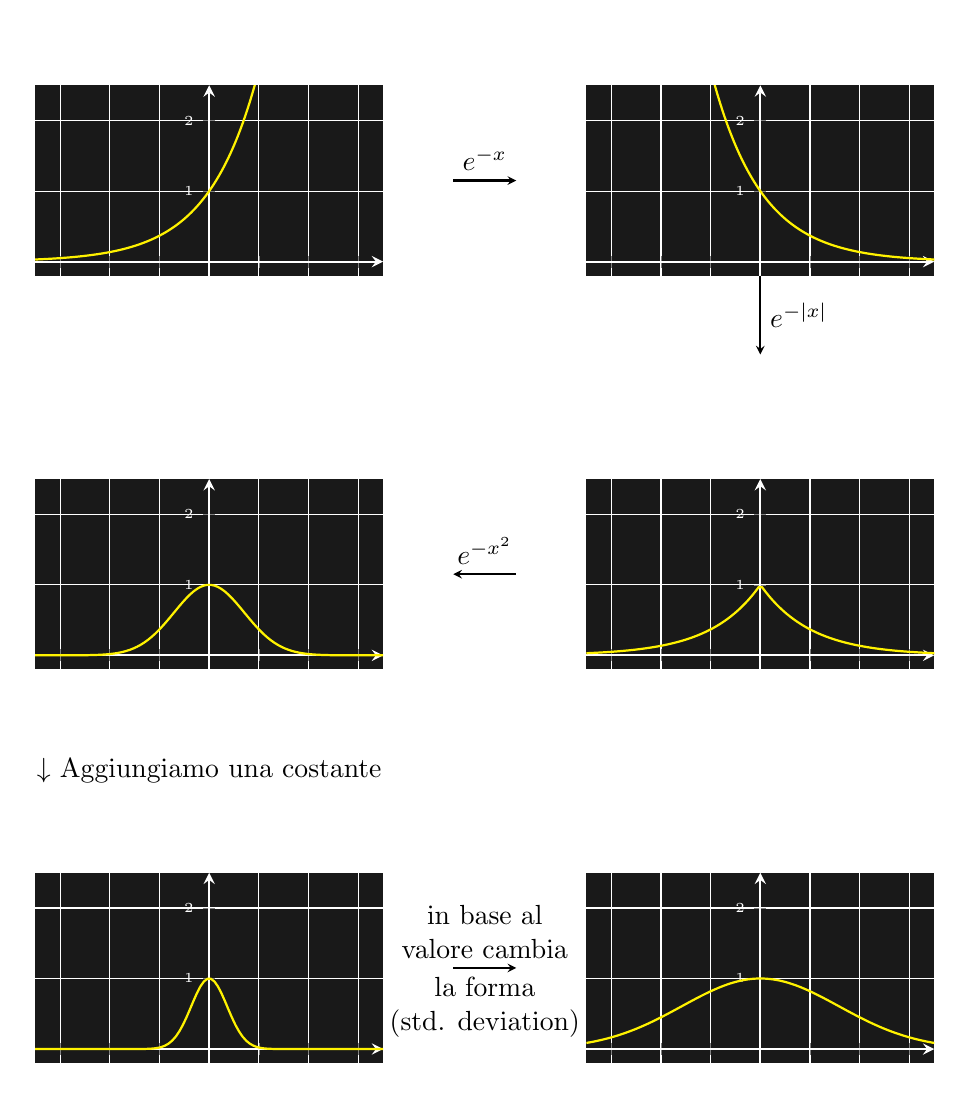
\begin{tikzpicture}[>=stealth, thick]
    % RIGA 1 (Senza annidamento dei nodi!)
    \begin{axis}[name=p1, at={(0,0)}, anchor=center, desmos, title={$e^x$}]
        \addplot[yellow, thick, domain=-3.5:1.2] {exp(x)};
    \end{axis}
    
    \begin{axis}[name=p2, at={(7cm,0)}, anchor=center, desmos, title={$e^{-x}$}]
        \addplot[yellow, thick, domain=-1.2:3.5] {exp(-x)};
    \end{axis}
    
    \draw[->] (3.1, 0) -- node[above]{$e^{-x}$} (3.9, 0);
    \draw[->] (p2.south) -- node[right]{$e^{-|x|}$} ++(0, -1);

    % RIGA 2
    \begin{axis}[name=p4, at={(7cm,-5cm)}, anchor=center, desmos, title={$e^{-|x|}$}]
        \addplot[yellow, thick, domain=-3.5:3.5] {exp(-abs(x))};
    \end{axis}
    
    \begin{axis}[name=p3, at={(0,-5cm)}, anchor=center, desmos, title={$e^{-x^2}$}]
        \addplot[yellow, thick, domain=-3.5:3.5] {exp(-x^2)};
    \end{axis}
    
    \draw[<-] (3.1, -5) -- node[above]{$e^{-x^2}$} (3.9, -5);
    
    % RIGA 3
    \node[align=center] at (0, -7.5) {$\downarrow$ Aggiungiamo una costante};
    
    \begin{axis}[name=p5, at={(0,-10cm)}, anchor=center, desmos, title={$e^{-cx^2}$}]
        \addplot[yellow, thick, domain=-3.5:3.5] {exp(-3.84*x^2)};
    \end{axis}
    
    \begin{axis}[name=p6, at={(7cm,-10cm)}, anchor=center, desmos, title={$e^{-cx^2}$}]
        \addplot[yellow, thick, domain=-3.5:3.5] {exp(-0.2*x^2)};
    \end{axis}
    
    \draw[->] (3.1, -10) -- node[align=center, above]{in base al\\valore cambia} node[align=center, below]{la forma\\(std. deviation)} (3.9, -10);

\end{tikzpicture}
\end{center}

$e$ non è speciale, perché per le proprietà delle potenze appartengono tutte alla stessa famiglia di funzioni.
Usiamo $e$ perché è leggibile.

\vspace{0.5cm}

\begin{center}
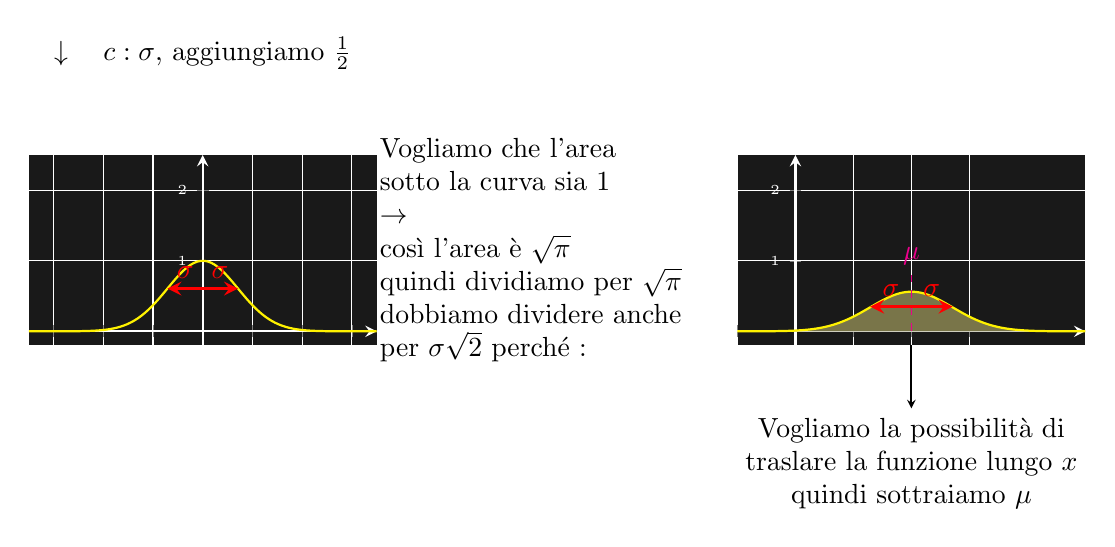
\begin{tikzpicture}[>=stealth, thick]
    % Sostituzione di c con sigma
    \node[align=center] at (0, 2.5) {$\downarrow \quad c : \sigma$, aggiungiamo $\frac{1}{2}$};
    
    % GRAFICO 1 (Con Nodi Interni FUNZIONANTI perché l'asse non è dentro un altro nodo)
    \begin{axis}[name=p7, at={(0,0)}, anchor=center, desmos, title={$e^{-\frac{1}{2}(x/\sigma)^2}$}]
        \addplot[yellow, thick, domain=-3.5:3.5] {exp(-0.5*(x/0.71)^2)};
        \draw[<->, red, very thick] (axis cs:-0.71, 0.606) -- (axis cs:0.71, 0.606);
        \node[red, above] at (axis cs:-0.35, 0.606) {$\sigma$};
        \node[red, above] at (axis cs:0.35, 0.606) {$\sigma$};
    \end{axis}
    
    % Testo centrale per la normalizzazione
    \node[align=left, text width=4.5cm] at (4.5, 0) {
        Vogliamo che l'area\\sotto la curva sia 1\\
        $\rightarrow$\\
        così l'area è $\sqrt{\pi}$\\
        quindi dividiamo per $\sqrt{\pi}$\\
        dobbiamo dividere anche\\
        per $\sigma\sqrt{2}$ perché :
    };
    
    % GRAFICO 2 (Traslato)
    \begin{axis}[name=p8, at={(9cm, 0)}, anchor=center, desmos, title={$\frac{1}{\sigma\sqrt{2\pi}}e^{-\frac{1}{2}\left(\frac{x-\mu}{\sigma}\right)^2}$ \quad $\mu=2.00$}, xmin=-1, xmax=5]
        \addplot[yellow, thick, fill=yellow!40!black, domain=-1:5] {1/(0.71*sqrt(2*pi)) * exp(-0.5*((x-2)/0.71)^2)};
        \draw[dashed, magenta] (axis cs:2, 0) -- (axis cs:2, 0.8);
        \node[magenta, above] at (axis cs:2, 0.8) {$\mu$};
        \draw[<->, red, very thick] (axis cs:1.29, 0.35) -- (axis cs:2.71, 0.35);
        \node[red, above] at (axis cs:1.65, 0.35) {$\sigma$};
        \node[red, above] at (axis cs:2.35, 0.35) {$\sigma$};
    \end{axis}
    
    \draw[->] (p8.south) -- ++(0,-0.8) node[below, align=center]{Vogliamo la possibilità di\\traslare la funzione lungo $x$\\quindi sottraiamo $\mu$};

\end{tikzpicture}
\end{center}

Più la media $\mu$ è grande, più la funzione si muove a dx.

La media è $\mathrm{mean} = \mu \cdot N$ \\
La std dev è $\mathrm{std\ dev} = \sigma \cdot \sqrt{N}$

Se prendiamo la somma di vari eventi $(X_1 + X_2 + \dots + X_N)$ e sottraiamo la media $N \cdot \mu$, stiamo centrando la "curva" a 0.
Se dividiamo per la std deviation riscala le unità cosicché la $\mathrm{std\ dev} = 1$.

\begin{equation}
\frac{(X_1 + \dots + X_N) - N\mu}{\sigma \cdot \sqrt{N}}
\end{equation}

Questa formula risponde alla domanda: \textit{"quante STD deviation è lontana dalla media $X_1 + \dots + X_N$?"}
Con la somma di 50 eventi, qualsiasi PDF tende alla curva Gaussiana.

\newpage
\subsection{Andamenti di PDF Gaussiane (Caratterizzazione marginale)}

Riproduciamo graficamente il comportamento della funzione di densità di probabilità di una variabile Gaussiana $X \sim \mathcal{N}(\mu_X, \sigma_X^2)$ al variare della media (traslazione orizzontale) e della varianza (apertura a campana).

\begin{center}
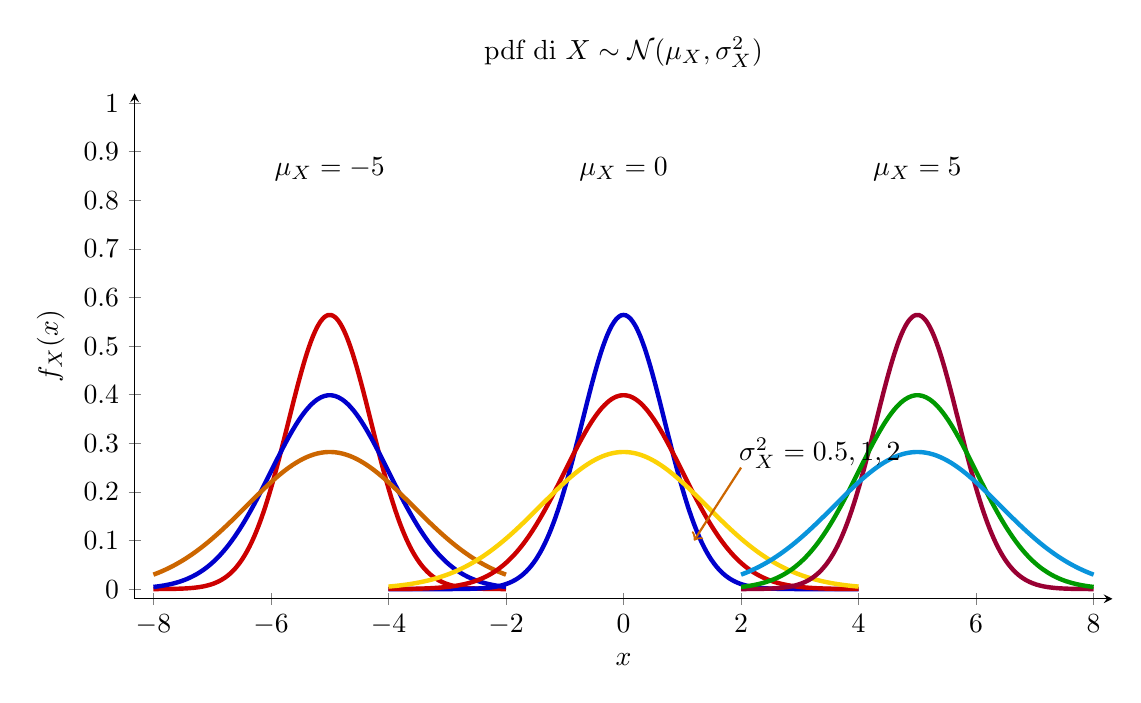
\begin{tikzpicture}
    \begin{axis}[
        width=14cm, height=8cm,
        xlabel={$x$},
        ylabel={$f_X(x)$},
        title={pdf di $X \sim \mathcal{N}(\mu_X, \sigma_X^2)$},
        xmin=-8, xmax=8,
        ymin=0, ymax=1,
        ytick={0, 0.1, 0.2, 0.3, 0.4, 0.5, 0.6, 0.7, 0.8, 0.9, 1},
        xtick={-8, -6, -4, -2, 0, 2, 4, 6, 8},
        axis lines=left,
        enlarge x limits=0.02,
        enlarge y limits=0.02,
        every axis plot/.append style={ultra thick, smooth, samples=100}
    ]
        
        % Gruppo mu = -5
        \addplot[red!80!black, domain=-8:-2] {1/(sqrt(0.5)*sqrt(2*pi)) * exp(-((x+5)^2)/(2*0.5))};
        \addplot[blue!80!black, domain=-8:-2] {1/(1*sqrt(2*pi)) * exp(-((x+5)^2)/(2*1))};
        \addplot[orange!80!black, domain=-8:-2] {1/(sqrt(2)*sqrt(2*pi)) * exp(-((x+5)^2)/(2*2))};
        \node[above] at (axis cs:-5, 0.82) {$\mu_X=-5$};
        
        % Gruppo mu = 0
        \addplot[blue!80!black, domain=-4:4] {1/(sqrt(0.5)*sqrt(2*pi)) * exp(-((x-0)^2)/(2*0.5))};
        \addplot[red!80!black, domain=-4:4] {1/(1*sqrt(2*pi)) * exp(-((x-0)^2)/(2*1))};
        \addplot[yellow!70!orange, domain=-4:4] {1/(sqrt(2)*sqrt(2*pi)) * exp(-((x-0)^2)/(2*2))};
        \node[above] at (axis cs:0, 0.82) {$\mu_X=0$};
        
        % Gruppo mu = 5
        \addplot[purple!80!black, domain=2:8] {1/(sqrt(0.5)*sqrt(2*pi)) * exp(-((x-5)^2)/(2*0.5))};
        \addplot[green!60!black, domain=2:8] {1/(1*sqrt(2*pi)) * exp(-((x-5)^2)/(2*1))};
        \addplot[cyan!80!blue, domain=2:8] {1/(sqrt(2)*sqrt(2*pi)) * exp(-((x-5)^2)/(2*2))};
        \node[above] at (axis cs:5, 0.82) {$\mu_X=5$};
        
        % Annotazione per le Varianze (frecce che indicano la larghezza)
        \draw[<-, thick, orange!80!black] (axis cs: 1.2, 0.1) -- (axis cs: 2, 0.25);
        \node[right] at (axis cs: 1.8, 0.28) {$\sigma_X^2 = 0.5, 1, 2$};

    \end{axis}
\end{tikzpicture}
\end{center}